\documentclass[10pt,paper=letter]{scrartcl}
\usepackage[alttitle]{cjquines}

\begin{document}

\title{VCSMS PRIME}
\subtitle{Program for Inducing Mathematical Excellence}
\author{Session 5: Trigonometry}
\date{September 28, 2017}

\maketitle
\setlength{\unitlength}{1in}
\begin{picture}(0,0)
  \put(5.5,0.5){\hbox{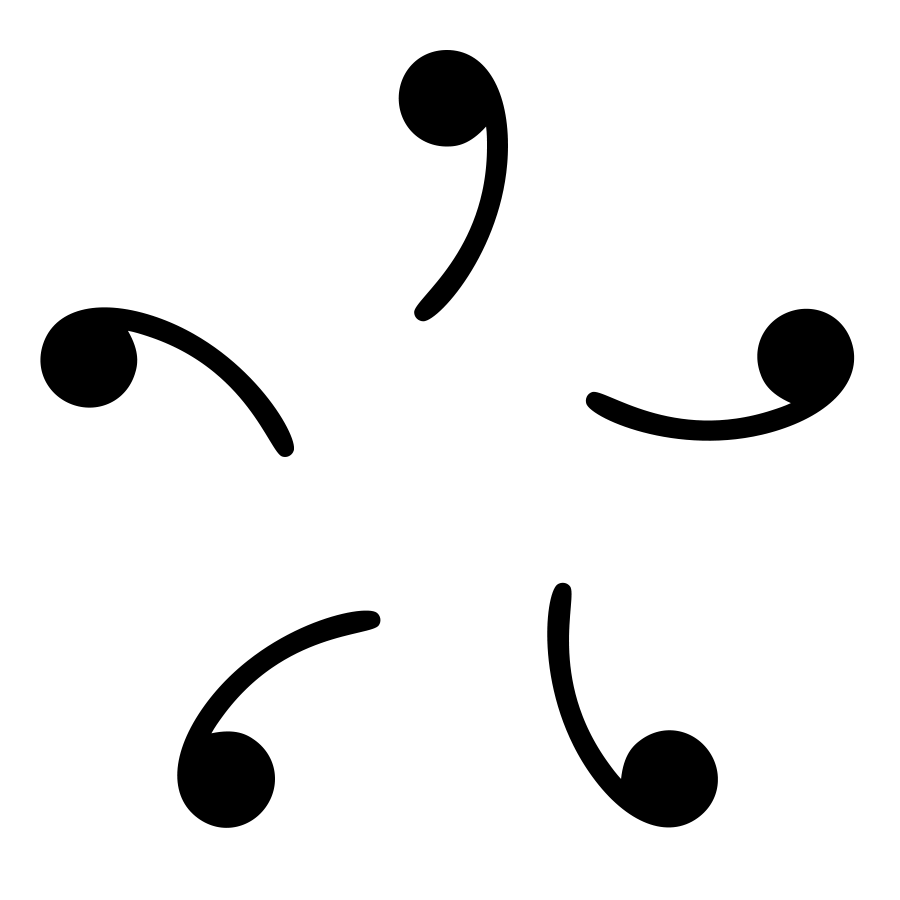
\includegraphics[width=0.9in]{logo.png}}}
\end{picture}
\vspace{-3.5em}

\subsubsection*{Lecture problems}

\begin{enumerate}
  \item (AIME 1995/7) Given $(1 + \sin t)(1 + \cos t) = \frac54$, find $(1 - \sin t)(1 - \cos t)$.
  \item (QI9) Evaluate the following sum: $1 + \cos\frac\pi3 + \cos\frac{2\pi}3 + \cos\frac{3\pi}3 + \cdots + \cos\frac{2016\pi}3.$
  \item (Huang\footnote{From Complex Numbers in Trigonometry, \url{https://aops.com/community/c6h609795}. Read it, it's good.}) Divide $\sin3x\del{2\cos2x - 1}$ by $\sin x\del{2 \cos 4x + 1}$ and simplify.
  \item (AIME 1996/10) Find the smallest positive integer solution to $\tan 19x\dg = \dfrac{\cos 96\dg + \sin 96\dg}{\cos 96\dg - \sin 96\dg}$.
  \item (AI6) Find the exact value of $\tan^{-1} \del{\frac{1}{2}} + \tan^{-1} \del{\frac{1}{5}} + \tan^{-1} \del{\frac{1}{8}}.$
  \item (Morrie's Law) Simplify $\cos20\dg\cos40\dg\cos80\dg$.
  \item Find the exact value of $\cos{\pi/5}$.
  \item (PEM 2016/10) Find the ratio of $\sin 1\dg + \sin 2\dg + \cdots + \sin 44\dg$ to $\cos 1\dg + \cos 2\dg + \cdots + \cos44\dg$.
  \item (Stewart's Theorem) In triangle $ABC$, point $D$ is on line $BC$. Let $AD = d, BD = m$ and $CD = n$. Then $man + dad = bmb + cnc$.
\end{enumerate}

\subsubsection*{As ratios of sides}

\begin{itemize}
  \item In terms of triangles: sine, cosine, tangent, secant, cosecant, cotangent, are ratios of sides. Example: find $\tan \alpha$ given $\sin \alpha = \frac12$. This is the classical development in classroom math.
  \item Values for special angles: $30\dg, 45\dg, 60\dg$ can be derived from special right triangles $30\dg-60\dg-90\dg$ (equilateral triangle), and $45\dg-45\dg-90\dg$ (square). We can get $0\dg$ and $90\dg$ from reasoning.
  \item Identities: cofunctions, Pythagorean identities.
  \item Problem 1: Abuse symmetry: replace sums and products with variables. Pythagorean identity.
\end{itemize}

\subsubsection*{As lengths in a circle}

\begin{itemize}
  \item In terms of circles: the functions are lengths in the unit circle: $\del{\sin\theta, \cos\theta}$. Tangent is the length of the tangent to $x$-axis, cotangent is length to $y$-axis. Secant and cosecant are $x$ and $y$ intercepts.
  \item Problem 2: Radians are more natural than degrees: $2\pi$ radians is $360\dg$.
  \item Identities: reflection over $0, \frac\pi4, \frac\pi2$, shifts by $\frac\pi2, \pi, 2\pi$, Pythagorean identities, $\csc^2\theta + \sec^2\theta = \del{\cot\theta + \tan\theta}^2$.
\end{itemize}

\subsubsection*{As complex numbers}

\begin{itemize}
  \item Euler's identity says $e^{ix} = \cos x + i \sin x$. Cosine is the real part and sine is the imaginary part.
  \item If $z = e^{ix}$ then $1/z = e^{-ix}$. We can state $\cos x$ and $\sin x$ in terms of $z$ only. Also, by de Moivre, $\del{e^{ix}}^n = \cos nx + i \sin nx$. We can find $\cos nx$ and $\sin nx$ in terms of $z$ only.
  \item Identities: reflection, Pythagorean identities.
  \item Problem 3: Let $z = e^{ix}$. Substitute sine and cosine. Everything cancels nicely.
\end{itemize}

\newpage

\subsubsection*{Sum and difference}

\begin{itemize}
  \item Fundamental is $\sin(x + y)$. Many derivations: stick two right triangles with angles $x$, $y$ and common side and find the area; use the unit circle and rotate; Euler's identity.
  \item Derive $\sin\del{x \pm y}, \cos\del{x \pm y}, \tan\del{x \pm y}, \cot\del{x \pm y}$. Triple tangent formula: $x + y + z = \pi$ iff $\tan x + \tan y + \tan z = \tan x \tan y \tan z$.
  \item Problem 4: Inspired by tangent sum formula. Force tangent by dividing by $\cos 96\dg$ and $\tan 45\dg = 1$. 
  \item Inverses for trigonometric functions exist. Derive $\tan^{-1} x \pm \tan^{-1} y$, $\cot^{-1} x \pm \cot^{-1} y$ by subtituting in the sum and difference formulas.
  \item Problem 5: The shortcut for $\tan^{-1}(p_1/q_1) + \tan^{-1}(p_2/q_2)$ is ``cross multiply and add for numerator, product of denominators minus product of numerators for denominator.''
  \item Derive $\sin 2x$. Write $\cos 2x$ in three ways using Pythagorean identity, and use that to derive half-angle formulas. (Sine is minus, same as in complex numbers.) There is also derivation with Euler's formula.
  \item Problem 6: The doubling inspires us to force double angle formula. Let expression be $x$ and multiply both sides by $2\sin 20\dg$. (Interestingly, $\tan20\dg\tan40\dg\tan80\dg = \tan60\dg$.)
  \item Problem 7: This is important. Let $a = \cos{\pi/5}$ and $b = \cos{2\pi/5}$. Then use double angle formulas on $a$ and $b$, but $\cos{4\pi/5} = -\cos{\pi/5} = -a$. 
\end{itemize}

\subsubsection*{Prosthaphaeresis}

\begin{itemize}
  \item Greek \emph{prosthesis} means addition, \emph{aphaeresis} means subtraction. Which is how you derive them: $\cos x \cos y, \sin x\sin y, \sin x \cos y$ by cancelling out $\cos(x + y)$ and $\cos(x - y)$, etc.
  \item Reverse formulas: find $\sin x \pm \sin y$ by reversing the prosthaphaeresis formulas. As in, let $x' = x - y$ and let $y' = x + y$ and rewrite.
  \item Problem 8: Looks like arithmetic sequence. We did arithmetic sequence by pairing up opposite terms. Here, we pair $\sin 1\dg$ and $\sin 44\dg$ and use sum-to-product, etc. Everything cancels.
\end{itemize}

\subsubsection*{Laws}

\begin{itemize}
  \item Extended law of sines: draw the circumradius and use the definition of sine. Law of cosines: drop an altitude use the Pythagorean theorem twice.
  \item Problem 9: Apply law of cosines twice: on $\triangle ABD$ and $\triangle BCD$.
\end{itemize}

\subsubsection*{As functions}

\begin{itemize}
  \item Sine and cosine: domain is $\RR$, range is $\cbr{-1, 1}$. Period $2\pi$. Graphs are translations of each other.
  \item Cosecant and secant graphs are like a bunch of parabolas. Cosecant domain is $\RR - \cbr{n\pi, n \in \ZZ}$ and secant domain is $\RR - \cbr{(2n+1)\pi/2, n \in \ZZ}$. Range is $(-\infty, -1] \cup [1, \infty)$.
  \item Tangent and cotangent: tangent domain is $\RR - \cbr{(2n+1)\pi/2, n \in \ZZ}$ and cotangent domain is $\RR - \cbr{n\pi, n \in \ZZ}$. Range is $\RR$.
  \item Inverse functions: arcsin and arccos are domain $[-1, 1]$. Arcsin has range $\cbr{-\pi/2, \pi/2}$, arccos has range $\cbr{0, \pi}$. Arctan has domain $\RR$ and range $\cbr{-\pi/2, \pi/2}$: it maps the whole real line onto a finite interval.
  \item This means we need to be careful in solving equations like $\sin x = 1/2$, because there are infinitely many solutions. Also, $\sin^{-1} x + \cos^{-1} x = \pi/2$ and stuff like $\sin(\cos^{-1} x) = \sqrt{1 - x^2}$.
\end{itemize}

\newpage

\begin{center}
  \begin{minipage}{.45\textwidth}
    \begin{center}
      \def\arraystretch{3}
      \setlength{\tabcolsep}{12pt}
      \begin{tabular}{c|c|c|c|c}
        deg & rad & sin & cos & tan \\ \hline
        $0\dg$ & $0$ &  &  &  \\ \hline
        $15\dg$ & $\dfrac\pi{12}$ &  &  &  \\ \hline
        $18\dg$ & $\dfrac\pi{10}$ &  &  &  \\ \hline
        $22.5\dg$ & $\dfrac\pi8$ &  &  &  \\ \hline
        $30\dg$ & $\dfrac\pi6$ &  &  &
      \end{tabular}
    \end{center}
  \end{minipage}
  \begin{minipage}{.45\textwidth}
    \begin{center}
      \def\arraystretch{3}
      \setlength{\tabcolsep}{12pt}
      \begin{tabular}{c|c|c|c|c}
        deg & rad & sin & cos & tan \\ \hline
        $36\dg$ & $\dfrac\pi5$ &  &  &  \\ \hline
        $45\dg$ & $\dfrac\pi4$ &  &  &  \\ \hline
        $60\dg$ & $\dfrac\pi3$ &  &  &  \\ \hline
        $90\dg$ & $\dfrac\pi2$ &  &  &  \\ \hline
        $180\dg$ & $\pi$ &  &  &
      \end{tabular}
    \end{center}
  \end{minipage}
\end{center}
\vspace{1em}
\openup 1em

\begin{multicols}{2}

  \noindent\textbf{Pythagorean identity:} $\sin^2 \theta + \cos^2 \theta = \rule{1cm}{0.15mm}$\\Dividing by $\sin^2 \theta$ gives: $\rule{4cm}{0.15mm}$\\Dividing by $\cos^2 \theta$ gives: $\rule{4cm}{0.15mm}$

  \noindent\textbf{Sum and difference:}\\
  $\sin\del{x \pm y} = \rule{6cm}{0.15mm}$\\
  $\cos\del{x \pm y} = \rule{6cm}{0.15mm}$\vspace{0.75em}\\
  $\tan\del{x \pm y} = \rule{6cm}{0.15mm}$\vspace{0.75em}\\
  $\cot\del{x \pm y} = \rule{6cm}{0.15mm}$

  \noindent\textbf{Arctans:}\vspace{0.75em}\\
  $\tan^{-1}x + \tan^{-1}y = \rule{5cm}{0.15mm}$\vspace{0.75em}\\
  $\cot^{-1}x + \cot^{-1}y = \rule{5cm}{0.15mm}$\vspace{0.75em}\\
  $\tan^{-1}\dfrac{p_1}{q_1} + \tan^{-1}\dfrac{p_2}{q_2} = \rule{4.7cm}{0.15mm}$

  \noindent\textbf{Half-angle:}\vspace{0.75em}\\
  $\sin{\dfrac{x}2} = \rule{6cm}{0.15mm}$\vspace{0.75em}\\
  $\cos{\dfrac{x}2} = \rule{6cm}{0.15mm}$

  \columnbreak

  \noindent\textbf{Double angle:}\\
  $\sin{2x} = \rule{6cm}{0.15mm}$\\
  $\cos{2x} = \rule{6cm}{0.15mm}$\vspace{0.75em}\\
  $\tan{2x} = \rule{6cm}{0.15mm}$\vspace{0.75em}\\
  $\cot{2x} = \rule{6cm}{0.15mm}$

  \noindent\textbf{Product-to-sum:}\\
  $2\cos x \cos y = \rule{5.5cm}{0.15mm}$\\
  $2\sin x \sin y = \rule{5.5cm}{0.15mm}$\\
  $2\sin x \cos y = \rule{5.5cm}{0.15mm}$

  \noindent\textbf{Sum-to-product:}\vspace{0.75em}\\
  $\sin x \pm \sin y = \rule{5.5cm}{0.15mm}$\vspace{0.75em}\\
  $\cos x + \cos y = \rule{5.5cm}{0.15mm}$\vspace{0.75em}\\
  $\cos x - \cos y = \rule{5.5cm}{0.15mm}$\vspace{1em}

 \noindent
  \textbf{Law of sines:} $\rule{5.5cm}{0.15mm}$\vspace{1em}\\
  \textbf{Law of cosines:} $\rule{5cm}{0.15mm}$.
\end{multicols}

\end{document}
